%% ============================================================
%%  Introduction to Spatial Statistics — REU Undergraduate Version
%%  Compile: pdflatex spatial_simple.tex  (twice)
%% ============================================================
\documentclass[aspectratio=169, 12pt]{beamer}

\usetheme{default}
\usecolortheme{whale}
\usefonttheme{professionalfonts}
\setbeamertemplate{navigation symbols}{}
\setbeamertemplate{itemize items}[circle]
\setbeamertemplate{footline}[frame number]

\definecolor{spatblue}{RGB}{31,73,125}
\definecolor{spataccent}{RGB}{0,114,178}
\definecolor{spatlightblue}{RGB}{214,234,248}
\definecolor{spatgray}{RGB}{90,90,90}
\definecolor{spatgreen}{RGB}{0,120,60}
\definecolor{spatred}{RGB}{180,40,40}
\definecolor{HH}{RGB}{215,48,39}
\definecolor{LL}{RGB}{69,117,180}
\definecolor{HL}{RGB}{252,141,89}
\definecolor{LH}{RGB}{145,191,219}

\setbeamercolor{frametitle}{bg=spatblue, fg=white}
\setbeamercolor{title}{bg=spatblue, fg=white}
\setbeamercolor{section in head/foot}{bg=spatblue}
\setbeamercolor{palette primary}{bg=spatblue, fg=white}
\setbeamercolor{palette secondary}{bg=spataccent, fg=white}
\setbeamercolor{palette tertiary}{bg=spatblue!80, fg=white}
\setbeamercolor{block title}{bg=spataccent, fg=white}
\setbeamercolor{block title alerted}{bg=spatred, fg=white}
\setbeamercolor{block title example}{bg=spatgreen, fg=white}
\setbeamercolor{alerted text}{fg=spatred}

\usepackage{amsmath}
\usepackage{booktabs}
\usepackage{xcolor}
\usepackage{listings}
\usepackage{tikz}
\usetikzlibrary{shapes.geometric, arrows.meta, positioning}

\lstdefinestyle{Rstyle}{
  language=R,
  basicstyle=\ttfamily\small,
  keywordstyle=\color{spatblue}\bfseries,
  commentstyle=\color{spatgray}\itshape,
  stringstyle=\color{spatgreen},
  backgroundcolor=\color{spatlightblue!40},
  frame=single, framerule=0.4pt,
  rulecolor=\color{spataccent},
  breaklines=true,
  showstringspaces=false,
  tabsize=2, xleftmargin=6pt, xrightmargin=6pt,
  aboveskip=4pt, belowskip=4pt,
  morekeywords={library,data,mutate,ggplot,geom_sf,aes,scale_fill_viridis_c,
    labs,theme_void,theme,poly2nb,nb2listw,lag.listw,moran.test,moran.mc,
    localmoran,case_when,variogram,fit.variogram,vgm,krige,st_read,st_crs,
    st_as_sf,st_coordinates,st_centroid,glimpse,summary,plot,
    coordinates,proj4string,gridded,CRS}
}
\lstset{style=Rstyle}

\newcommand{\pkg}[1]{\texttt{\color{spataccent}#1}}
\newcommand{\discuss}[1]{\begin{alertblock}{Discuss}\textit{#1}\end{alertblock}}

\title[Spatial Statistics]{Introduction to Spatial Statistics}
\subtitle{NSF REU Bootcamp - Last Day!}
\author{Monnie McGee, PhD}
\institute{Southern Methodist Universtiy}
\date{\today}

%% ============================================================
\begin{document}
%% ============================================================

\begin{frame}
  \titlepage
\end{frame}

%% ── PART 1 ──────────────────────────────────────────────────
\begin{frame}{The Big Idea}
  \begin{center}
    \Large\itshape
    ``Near things are more related\\
    than distant things.''\\[0.6em]
    \normalsize\upshape\textbf{--- Waldo Tobler, 1970}
  \end{center}
  \vspace{0.8em}
  \begin{block}{What this means for statistics}
    \begin{itemize}
      \item Most stats methods assume observations are \textbf{independent}
      \item Spatial data breaks that assumption --- nearby locations tend to look similar
      \item We call this \alert{spatial autocorrelation}
      \item Ignoring it leads to misleading $p$-values and conclusions
    \end{itemize}
  \end{block}
\end{frame}

% =================================================

\begin{frame}{Three Kinds of Spatial Data}
  \vspace{0.3em}
  \begin{columns}[T]
    \begin{column}{0.32\textwidth}
      \centering
      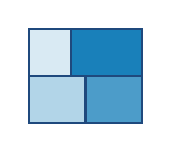
\begin{tikzpicture}[scale=0.6]
        \draw[fill=spataccent!30, draw=spatblue, thick] (0,0) rectangle (1.2,1);
        \draw[fill=spataccent!70, draw=spatblue, thick] (1.2,0) rectangle (2.4,1);
        \draw[fill=spataccent!15, draw=spatblue, thick] (0,1) rectangle (0.9,2);
        \draw[fill=spataccent!90, draw=spatblue, thick] (0.9,1) rectangle (2.4,2);
      \end{tikzpicture}\\[0.5em]
      \textbf{Areal}\\[0.3em]
      \small Values attached to polygons\\[0.5em]
      \footnotesize\textit{Counties, zip codes, census tracts}
    \end{column}
    \begin{column}{0.32\textwidth}
      \centering
      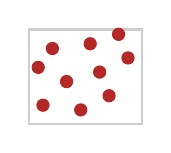
\begin{tikzpicture}[scale=0.6]
        \draw[draw=spatgray!30, thick] (0,0) rectangle (2.4,2);
        \foreach \x/\y in {0.3/0.4, 0.5/1.6, 0.8/0.9, 1.1/0.3,
                            1.3/1.7, 1.5/1.1, 1.7/0.6, 2.1/1.4,
                            0.2/1.2, 1.9/1.9}
          \fill[spatred] (\x,\y) circle (4pt);
      \end{tikzpicture}\\[0.5em]
      \textbf{Point process}\\[0.3em]
      \small Locations of events\\[0.5em]
      \footnotesize\textit{Disease cases, earthquakes, crimes}
    \end{column}
    \begin{column}{0.32\textwidth}
      \centering
      
\begin{tikzpicture}[scale=0.6]
        \foreach \x/\y/\c in {0.3/0.3/20, 0.9/1.5/60, 1.5/0.6/45,
                                2.0/1.8/80, 0.6/1.0/50, 1.2/0.2/30,
                                1.8/1.1/70, 0.3/1.8/55}{
          \fill[spatgreen!\c!white] (\x,\y) circle (7pt);
          \fill[spatgreen!\c!black, opacity=0.5] (\x,\y) circle (5pt);
        }
      \end{tikzpicture}\\[0.5em]
      \textbf{Geostatistical}\\[0.3em]
      \small Continuous surface, sampled at points\\[0.5em]
      \footnotesize\textit{Soil chemistry, air quality monitors}
    \end{column}
  \end{columns}
  \vspace{0.6em}
  \begin{center}
    \small We will work through a real example of each type today.
  \end{center}
\end{frame}

%% ── PART 2 ──────────────────────────────────────────────────
\begin{frame}{Part 1: Areal Data --- NC SIDS}
  \begin{columns}[t]
    \begin{column}{0.55\textwidth}
      \textbf{Dataset: North Carolina SIDS}
      \begin{itemize}
        \item Sudden Infant Death Syndrome deaths
        \item 100 NC counties, 1974--1984
        \item Classic teaching dataset in spatial stats
        \item Built into the \pkg{spData} package
      \end{itemize}
      \vspace{0.6em}
      \textbf{Our question:}\\
      Are high SIDS rates \emph{clustered} in certain parts of the state, or are they scattered randomly?
    \end{column}
    \begin{column}{0.42\textwidth}
      \begin{exampleblock}{Compute a rate}
        \texttt{nc <- nc \textbar>\!\!\!>}\\
        \texttt{\ \ mutate(}\\
        \texttt{\ \ \ \ rate =}\\
        \texttt{\ \ \ \ \ \ SID74/BIR74*1000)}
        \vspace{0.3em}

        \small Deaths per 1,000 live births
      \end{exampleblock}
    \end{column}
  \end{columns}
\end{frame}
% =================================================
\begin{frame}[fragile]{Making a Choropleth Map}
  \begin{columns}[t]
    \begin{column}{0.52\textwidth}
\begin{lstlisting}
ggplot(nc) +
  geom_sf(
    aes(fill = sids_rate74),
    color = "white") +
  scale_fill_viridis_c(
    option = "magma") +
  theme_void()
\end{lstlisting}
      \vspace{0.4em}
      \small \textbf{Choropleth}: shade each polygon by its value. Darker = higher rate.
    \end{column}
    \begin{column}{0.45\textwidth}
      \discuss{Look at the map. Do high-rate counties seem to cluster together, or are they scattered randomly across the state?}
    \end{column}
  \end{columns}
\end{frame}

% =================================================

\begin{frame}{North Carolina Choropleth Map}

\centering
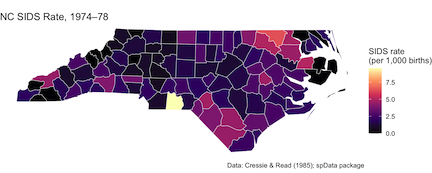
\includegraphics[scale=.8]{choroplethNC.png}

\end{frame}

% =================================================
\begin{frame}{Who Is a Neighbor?}
  \begin{block}{We need to define ``nearby'' formally}
    \textbf{Queen contiguity}: two counties are neighbors if they share \emph{any} boundary point (like a queen's move in chess).
  \end{block}
  \vspace{0.5em}
  \begin{columns}[c]
    \begin{column}{0.45\textwidth}
    \centering
      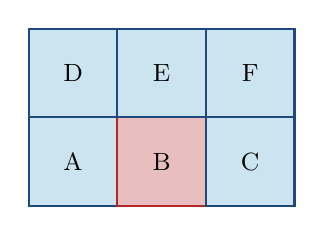
\begin{tikzpicture}[scale=0.75]
        \draw[fill=spataccent!20, draw=spatblue, thick] (0,0) rectangle (1.5,1.5) node[midway]{\small A};
        \draw[fill=spatred!30,    draw=spatred,  thick] (1.5,0) rectangle (3,1.5)   node[midway]{\small B};
        \draw[fill=spataccent!20, draw=spatblue, thick] (3,0) rectangle (4.5,1.5)   node[midway]{\small C};
        \draw[fill=spataccent!20, draw=spatblue, thick] (0,1.5) rectangle (1.5,3)   node[midway]{\small D};
        \draw[fill=spataccent!20, draw=spatblue, thick] (1.5,1.5) rectangle (3,3)   node[midway]{\small E};
        \draw[fill=spataccent!20, draw=spatblue, thick] (3,1.5) rectangle (4.5,3)   node[midway]{\small F};
      \end{tikzpicture}\\[0.3em]
      \small\textcolor{spatred}{B's neighbors: A, C, E (queen)}
    \end{column}
    \begin{column}{0.52\textwidth}
      \small Other options:
      \begin{itemize}
        \item \textbf{Rook}: shared edge only (not corners)
        \item \textbf{$k$-nearest neighbors}: closest $k$ centroids
        \item \textbf{Distance band}: all within $d$ km
      \end{itemize}
     \end{column}
  \end{columns}
     \pause
      \vspace{1em}
The choice matters --- it's a modeling decision!
\end{frame}
% =================================================
\begin{frame}[fragile]{Building the Neighbor Structure in R}
\begin{lstlisting}
# Define neighbors (queen contiguity)
nc_nb <- poly2nb(nc, queen = TRUE)

# Convert to weights (each row sums to 1)
nc_lw <- nb2listw(nc_nb, style = "W")

# The spatial lag: each county's neighbors' average
nc$sids_lag <- lag.listw(nc_lw, nc$sids_rate74)
\end{lstlisting}
  \vspace{0.5em}
  \begin{block}{Spatial lag, in plain English}
    For each county, compute the \textbf{average SIDS rate among its neighbors}.\\[4pt]
    If autocorrelation is present, a county's own rate and its neighbors' average should be correlated.
  \end{block}
\end{frame}

% =================================================

\begin{frame}[fragile]{The Moran Scatterplot}
\begin{lstlisting}
ggplot(nc, aes(x = sids_rate74, y = sids_lag)) +
  geom_point(color = "steelblue") +
  geom_smooth(method = "lm", color = "tomato") +
  labs(x = "County SIDS rate",
       y = "Neighbors' average rate")
\end{lstlisting}
  %\vspace{0.4em}
  \begin{columns}[t]
    \begin{column}{0.48\textwidth}
      \begin{block}{Reading the plot}
        \begin{itemize}
          \item \textbf{Positive slope}: nearby counties look similar \textrightarrow{} clustering
          \item \textbf{Flat}: no spatial pattern
          \item \textbf{Negative slope}: checkerboard pattern
        \end{itemize}
      \end{block}
    \end{column}
    \begin{column}{0.48\textwidth}
      \small The slope of that red line is \textbf{Moran's $I$}, the most common measure of spatial autocorrelation.
      \vspace{0.4em}

      Range: roughly $-1$ to $+1$\\
      (like a correlation coefficient, but for space)
    \end{column}
  \end{columns}
\end{frame}

% =================================================

\begin{frame}[fragile]{Testing: Is the Clustering Real?}
\begin{lstlisting}
# Analytical test
moran.test(nc$sids_rate74, nc_lw)
\end{lstlisting}

$$I = \frac{n}{\sum_{i}\sum_{j} w_{ij}} \cdot \frac{\sum_{i}\sum_{j} w_{ij}(x_i - \bar{x})(x_j - \bar{x})}{\sum_i (x_i - \bar{x})^2}$$
\vspace{.5em}
\begin{itemize}
\item $I \approx 0$: no spatial autocorrelation (random)
\item $I > 0$: positive autocorrelation (clusters of similar values)
\item $I < 0$: negative autocorrelation (checkerboard pattern)
\end{itemize}
\end{frame}

% =================================================

\begin{frame}[fragile]{Safer: Permutation Test}

Shuffle the map a large number of times

\begin{lstlisting}
set.seed(42)
moran.mc(nc$sids_rate74, nc_lw, nsim = 999)
\end{lstlisting}

  \vspace{0.4em}
  \begin{block}{How the permutation test works}
    \begin{enumerate}
      \item Randomly reassign the 100 SIDS rates to random counties
      \item Compute Moran's $I$ for that scrambled map
      \item Repeat 999 times to build a ``what if spatial pattern were random'' distribution
      \item Ask: is our observed $I$ unusual compared to those 999 values?
    \end{enumerate}
  \end{block}
\end{frame}

% =================================================

\begin{frame}{Where Are the Clusters? --- LISA}
  \begin{columns}[t]
    \begin{column}{0.50\textwidth}
      \textbf{Global Moran's $I$}: one number for the whole map.\\[0.5em]
      \textbf{LISA} (Local Indicators of Spatial Association): tells us \emph{where} clusters are.
      \vspace{0.6em}

      \begin{tabular}{@{}cl@{}}
        \textcolor{HH}{\rule{12pt}{12pt}} & \textbf{High--High}: hot spot\\[4pt]
        \textcolor{LL}{\rule{12pt}{12pt}} & \textbf{Low--Low}: cold spot\\[4pt]
        \textcolor{HL}{\rule{12pt}{12pt}} & \textbf{High--Low}: high outlier\\[4pt]
        \textcolor{LH}{\rule{12pt}{12pt}} & \textbf{Low--High}: low outlier\\[4pt]
        \textcolor{gray}{\rule{12pt}{12pt}} & Not significant\\
      \end{tabular}
    \end{column}
    \begin{column}{0.47\textwidth}
      \begin{exampleblock}{In R}
        \texttt{lisa <- localmoran(}\\
        \texttt{\ \ nc\$sids\_rate74, nc\_lw)}
      \end{exampleblock}
      \vspace{0.5em}
      \discuss{Where do hot spots appear on the NC map? Do they correspond to any geographic or demographic pattern you might expect?}
    \end{column}
  \end{columns}
\end{frame}

% =================================================

\begin{frame}{North Carolina LISA Map}

\centering
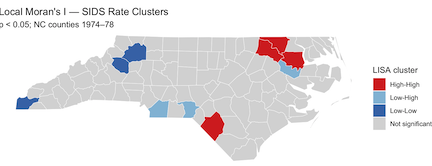
\includegraphics[scale=.8]{lisaNC.png}

\end{frame}


%% ── PART 3 ──────────────────────────────────────────────────
\begin{frame}{Part 2: Point Patterns --- Fiji Earthquakes}
  \begin{block}{The question}
    Are the events \textbf{clustered}, \textbf{random}, or \textbf{regular}?
  \end{block}
  \vspace{0.5em}
  \begin{columns}[T]
    \begin{column}{0.30\textwidth}
      \centering\textbf{Clustered}\\[4pt]
      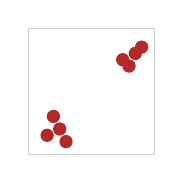
\begin{tikzpicture}[scale=0.8]
        \draw[draw=spatgray!30] (0,0) rectangle (2,2);
        \foreach \x/\y in {0.3/0.3,0.5/0.4,0.4/0.6,0.6/0.2,
                            1.5/1.5,1.7/1.6,1.6/1.4,1.8/1.7}
          \fill[spatred] (\x,\y) circle (3pt);
      \end{tikzpicture}
    \end{column}
    \begin{column}{0.30\textwidth}
      \centering\textbf{Random (CSR*)}\\[4pt]
      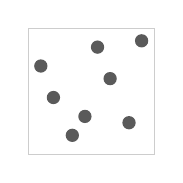
\begin{tikzpicture}[scale=0.8]
        \draw[draw=spatgray!30] (0,0) rectangle (2,2);
        \foreach \x/\y in {0.2/1.4,0.7/0.3,1.1/1.7,1.6/0.5,
                            0.4/0.9,1.3/1.2,1.8/1.8,0.9/0.6}
          \fill[spatgray] (\x,\y) circle (3pt);
      \end{tikzpicture}
    \end{column}
    \begin{column}{0.30\textwidth}
      \centering\textbf{Regular}\\[4pt]
      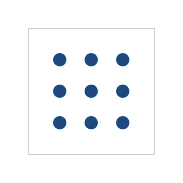
\begin{tikzpicture}[scale=0.8]
        \draw[draw=spatgray!30] (0,0) rectangle (2,2);
        \foreach \x in {0.5,1.0,1.5}
          \foreach \y in {0.5,1.0,1.5}
            \fill[spatblue] (\x,\y) circle (3pt);
      \end{tikzpicture}
    \end{column}
  \end{columns}
  \vspace{0.6em}
  \begin{center}
    Dataset: \texttt{quakes} (base R) --- 1,000 earthquakes near Fiji, magnitude $\geq 4$
  \end{center}
\end{frame}

\begin{frame}[fragile]{Visualizing Point Data: Kernel Density}
  \begin{columns}[t]
    \begin{column}{0.52\textwidth}
\begin{lstlisting}
# Raw points
ggplot(quakes,
  aes(x = long, y = lat)) +
  geom_point(alpha = 0.3)
\end{lstlisting}
      \begin{block}{Kernel density estimation}
        Place a smooth ``bump'' over each point. Add them all up. The result is a continuous surface showing \textbf{where events are most concentrated}.
      \end{block}
 \end{column}
 
 \begin{column}{0.45\textwidth}
\begin{lstlisting}
# Density surface
ggplot(quakes,
  aes(x = long, y = lat)) +
  stat_density_2d(
    aes(fill=after_stat(
          density)),
    geom="raster",
    contour=FALSE) +
  scale_fill_viridis_c(
    option="inferno")
\end{lstlisting}
    \end{column}
  \end{columns}
\end{frame}

% ===========================================
\begin{frame}{Cluster Patterns}
      \discuss{What pattern do you see? Why might earthquakes cluster near Fiji?}
      
      \begin{columns}
       \begin{column}{0.45\textwidth}
       \centering
       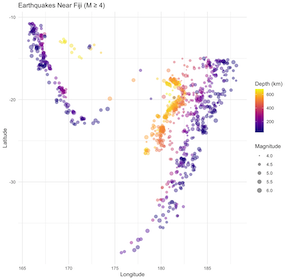
\includegraphics[scale=.6]{pointsEpicenters.png}
       \end{column}
        \begin{column}{0.45\textwidth}
        \centering
        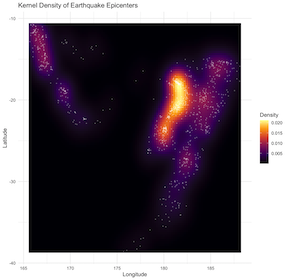
\includegraphics[scale=.6]{kdeEpicenters.png}
       \end{column}
      \end{columns}
\end{frame}

%% ── PART 4 ──────────────────────────────────────────────────
\begin{frame}{Part 3: Geostatistics --- Meuse River Soils}
  \begin{columns}[t]
    \begin{column}{0.55\textwidth}
      \textbf{Setup}
      \begin{itemize}
        \item 155 soil samples from the Meuse river floodplain (Netherlands)
        \item Measuring zinc concentration (ppm) at each point
        \item \textbf{Goal}: predict zinc everywhere, not just at sample locations
      \end{itemize}
      \vspace{0.5em}
      \textbf{Why not just take the average?}\\
      Zinc concentration isn't uniform --- it's higher near the river channel. We want a \emph{spatial} prediction.
    \end{column}
    \begin{column}{0.42\textwidth}
      \begin{exampleblock}{Load the data}
        \texttt{data("meuse", package="sp")}\\[4pt]
        \texttt{meuse\_sf\$log\_zinc <-}\\
        \texttt{\ \ log(meuse\_sf\$zinc)}
        \vspace{0.3em}

        \small Log-transform: zinc values are right-skewed
      \end{exampleblock}
    \end{column}
  \end{columns}
\end{frame}

% ===========================================

\begin{frame}{The Variogram: Does Similarity Decay with Distance?}
  \begin{columns}[c]
    \begin{column}{0.52\textwidth}
      \textbf{Key idea:} Nearby soil samples should have similar zinc levels. Far-apart samples should be less similar.
      \vspace{0.5em}

      The \textbf{variogram} plots:
      \begin{center}
        \textit{average squared difference between pairs of measurements}\\
        vs.\\
        \textit{distance between them}
      \end{center}
      If the curve rises then flattens, spatial correlation exists.
    \end{column}
    \begin{column}{0.45\textwidth}
      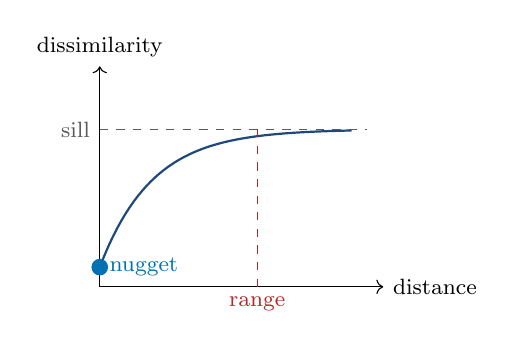
\begin{tikzpicture}[scale=1.0]
        \draw[->] (0,0) -- (3.6,0) node[right]{\footnotesize distance};
        \draw[->] (0,0) -- (0,2.8) node[above]{\footnotesize dissimilarity};
        \draw[thick, spatblue, domain=0:3.2, samples=60]
          plot (\x, {0.25 + 1.75*(1 - exp(-3*\x/2))});
        \draw[dashed, spatgray] (0,2.0) node[left]{\footnotesize sill} -- (3.4,2.0);
        \draw[dashed, spatred]  (2.0,0) node[below]{\footnotesize range} -- (2.0,2.0);
        \fill[spataccent] (0,0.25) circle (3pt)
          node[right]{\footnotesize \textcolor{spataccent}{nugget}};
      \end{tikzpicture}
      \vspace{0.3em}
      \footnotesize
      \textbf{Nugget}: residual variance at zero distance\\
      \textbf{Range}: correlation disappears beyond here\\
      \textbf{Sill}: total variance
    \end{column}
  \end{columns}
\end{frame}

% ===========================================

\begin{frame}[fragile]{Computing the Variogram in R}
\vspace{-.3em}
$$\gamma(h) = \frac{1}{2|N(h)|} \sum_{N(h)} [Z(s_i) - Z(s_j)]^2$$

where $N(h)$ is the set of pairs separated by distance $h$.

\begin{lstlisting}
# Step 1: compute empirical variogram
v_emp <- variogram(log_zinc ~ 1, data = meuse_sp)
plot(v_emp)
# Step 2: fit a model (spherical shape)
v_fit <- fit.variogram(v_emp,
           model = vgm(psill  = 0.6,
                       model  = "Sph",
                       range  = 900,
                       nugget = 0.05))
plot(v_emp, v_fit)
\end{lstlisting}
\end{frame}

% ===========================================
\begin{frame}{Empirical Variogram Interpretation}
  \discuss{Does your variogram level off? At roughly what distance? Is the nugget large or small relative to the sill?}
  
        \begin{columns}
       \begin{column}{0.45\textwidth}
       \centering
       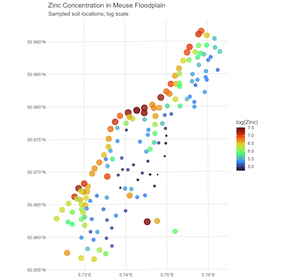
\includegraphics[scale=.6]{meuseData.png}
       \end{column}
        \begin{column}{0.45\textwidth}
        \centering
        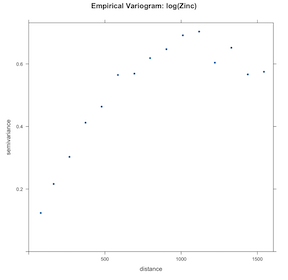
\includegraphics[scale=.6]{meuseVariogram.png}
       \end{column}
      \end{columns}
\end{frame}
% ===========================================

\begin{frame}[fragile]{Kriging: Spatial Interpolation}
  \begin{block}{What is kriging?}
    Predict zinc at any unsampled location by taking a \textbf{weighted
    average of nearby observations}. Closer samples get more weight.
    The variogram tells us exactly how to assign the weights.
  \end{block}
  \vspace{0.4em}
  \begin{columns}[t]
    \begin{column}{0.55\textwidth}
\begin{lstlisting}
krig_out <- krige(
  log_zinc ~ 1, # formula
  meuse_sp,     # sample data
  meuse.grid,   # predict here
  model = v_fit)# variogram
\end{lstlisting}
    \end{column}
    \begin{column}{0.42\textwidth}
      \small\textbf{Kriging gives you two maps:}
      \begin{itemize}
        \item \textbf{Prediction}: best estimate of zinc everywhere
        \item \textbf{Variance}: uncertainty of estimates,  lowest near sample points
      \end{itemize}
    \end{column}
  \end{columns}
\end{frame}

% ── Ordinary vs Universal kriging concept ───────────
\begin{frame}{Two Kinds of Kriging}
  \begin{columns}[t]
    \begin{column}{0.48\textwidth}
      \begin{block}{Ordinary Kriging}
        \texttt{log\_zinc \textasciitilde{} 1}\\[0.5em]
        Assumes the mean zinc concentration is \textbf{constant} across the whole study area.\\[0.5em]
        All spatial pattern is treated as random variation around that one global mean.
      \end{block}
      \vspace{0.4em}
      \small\textbf{Use when:} no obvious directional gradient in your map of raw data
    \end{column}
    \begin{column}{0.48\textwidth}
      \begin{block}{Universal Kriging}
        \texttt{log\_zinc \textasciitilde{} dist}\\[0.5em]
        Allows the mean to \textbf{vary} as a function of a covariate (here: distance to river).\\[0.5em]
        First removes the trend, then models spatial structure in what remains.
      \end{block}
      \vspace{0.4em}
      \small\textbf{Use when:} a clear gradient is visible, like zinc decreasing away from the river
    \end{column}
  \end{columns}
\end{frame}

% ── Why it matters ──────────────────────────────────
\begin{frame}{Why Does the Choice Matter?}
  \begin{columns}[t]
    \begin{column}{0.48\textwidth}
      \textbf{What goes wrong with ordinary kriging when there is a trend?}
      \begin{itemize}
        \item The variogram absorbs the trend into the sill
        \item Sill ends up \alert{inflated} above the true sample variance
        \item Spatial correlation structure is mis-estimated
        \item Predictions away from data can be biased
      \end{itemize}
      \vspace{0.4em}
      \small In our Meuse example: sill was 0.64 under \texttt{\textasciitilde{}1} but only 0.29 under \texttt{\textasciitilde{}dist}
    \end{column}
    \begin{column}{0.48\textwidth}
      \textbf{What universal kriging buys you:}
      \begin{itemize}
        \item Cleaner variogram fit closer to sample variance
        \item Shorter, more realistic range estimate
        \item Predictions that respect the physical gradient
        \item Lower prediction variance near the trend
      \end{itemize}
      \vspace{0.4em}
      \small In our example: range shrank from 897m to 729m once the river-distance trend was removed
    \end{column}
  \end{columns}
\end{frame}

% ── How to choose ───────────────────────────────────
\begin{frame}{How to Choose: A Simple Workflow}
  \begin{enumerate}
    \setlength\itemsep{0.7em}
    \item \textbf{Map your raw data first.} \\
      \small If you see a clear directional gradient, a trend is present.
    \item \textbf{Check: does the variogram sill match} \texttt{var(y)}? \\
      \small A sill much larger than the sample variance suggests a trend is inflating it.
    \item \textbf{If trend present}: fit \texttt{y \textasciitilde{} covariate} and recompute the variogram on the residuals.
    \item \textbf{Compare the two variograms.} \\
      \small The universal kriging variogram should have a lower sill and fit closer to the sample variance.
    \item \textbf{Use the matching formula in} \texttt{krige()}. \\
      \small Whatever formula you used in \texttt{variogram()}, use the same one in \texttt{krige()}.
  \end{enumerate}
\end{frame}

\begin{frame}{Practical Limitation of Universal Kriging}

\begin{alertblock}{Discuss}
    \itshape Universal kriging requires a covariate measured at every
    prediction location, not just at sample points. 
    \begin{itemize}
    \item What does that mean practically? 
    \item What do you need to have in hand before you can run  \texttt{krige()}?
    \end{itemize}
  \end{alertblock}
\end{frame}

%% ── WRAP-UP ─────────────────────────────────────────────────
\begin{frame}{What We Covered}
  \vspace{0.3em}
  \begin{tabular}{lll}
    \toprule
    \textbf{Data type} & \textbf{Key idea} & \textbf{Main tool}\\
    \midrule
    Areal (NC counties) & Spatial autocorrelation & Moran's $I$, LISA\\
    Point process (earthquakes) & Clustering vs.\ random & Kernel density\\
    Geostatistical (Meuse soils) & Predict at new locations & Kriging\\
    \bottomrule
  \end{tabular}
  \vspace{0.7em}
  \begin{block}{The thread running through all three}
    \textbf{Nearby things tend to be similar.} Each method uses that fact differently:
    \begin{itemize}
      \item Moran's $I$ --- \textit{measures} how similar neighbors are
      \item KDE --- \textit{visualizes} where events concentrate
      \item Kriging --- \textit{exploits} similarity to predict in new places
    \end{itemize}
  \end{block}
\end{frame}

% ===========================================

\begin{frame}{Exercises}
  \begin{block}{Exercise 1}
    Repeat the Moran's $I$ test for the 1979--84 SIDS period (\texttt{sid\_rate79}). Does clustering increase or decrease over time?
  \end{block}
  \vspace{0.4em}
  \begin{block}{Exercise 2}
    Switch to $k = 5$ nearest-neighbor weights instead of queen contiguity. How much does Moran's $I$ change?\\[4pt]
    \texttt{knn2nb(knearneigh(coords, k = 5))}
  \end{block}
  \vspace{0.4em}
  \begin{alertblock}{Challenge}
    Install \pkg{spatstat}. Convert \texttt{quakes} to a \texttt{ppp} object and compute the $L$-function. Is there evidence of clustering at short distances?
  \end{alertblock}
\end{frame}

% ===========================================

\begin{frame}{Discussion Questions}
  \begin{enumerate}
    \setlength\itemsep{1em}
    \item We found that high SIDS counties tend to cluster together. Does that \textit{prove} something spatial is causing it? What else could explain the pattern?

    \item The choice of neighbor definition (queen, $k$-NN, distance band) is a \textit{modeling decision}. What could go wrong if you choose poorly?

    \item Kriging is most uncertain far from sample points. If you could add 10 more soil samples to the Meuse study, where would you place them?

    \item All three methods assume spatial pattern is \textit{stationary}, which means that the pattern is the same everywhere. When might that fail?
  \end{enumerate}
\end{frame}

% ===========================================

\begin{frame}{Free Online References}
  \begin{center}
    Lovelace, Nowosad \& Muenchow --- \textit{Geocomputation with R}\\
    Bivand, Pebesma \& G\'{o}mez-Rubio --- \textit{Applied Spatial Data Analysis with R}\\
    Pebesma \& Bivand --- \textit{Spatial Data Science} (r-spatial.org/book)
  \end{center}
\end{frame}

\end{document}
